\chapter{An Optimal Controller for Biped Walking Using Neural Fields}
\label{ch:chp3}
\section{Introduction}
\label{sec:chp3-introduction}
This chapter introduces the Simplest Biped Walking problem, which will
be used onwards as the reference control problem. Approximations to
optimal linear state-feedback controllers for the Simplest Biped
Walking problem are found using numerical methods (genetic
algorithms), for each sub-region on a delimited state-space region. A
general architecture for the neural field controllers is presented,
and an structured strategy to implement non-linear (sliding-mode-like)
state-space controllers using the neural field-like controller
architecture is shown. Finally, an specific controller for biped
walking is developed and tested using the collected data, its behavior
is shown using a Poincar� section for the controlled biped dynamics,
and an stability analysis is provided.

\section{The Simplest Biped Walking Model}
\label{sec:chp3-simplest}

The Simplest Walking Model, presented by Garcia et
al. \cite{Garcia98simplest}, is an attempt to create the simplest
model that is capable of mimicking bipedal gait. It provides a
reference model to study the phenomena that allows walking in two
dimensions, and it has been further studied in terms of stability
\cite{Schwab01Basin} \cite{Das02Alternative}, swing-leg control
\cite{Wisse05How}, energy consumption in active walking
\cite{Kuo02Energetics}, walking on stairs \cite{Safa07Passive}, and
walking with an upper body \cite{Wisse04Passive}.

Here is used the model of Garcia et al., as modified by Wisse et
al. to allow control torques.
% \ref{fig:chp3-simplest}.

The 2D Biped Walking (yet to be simplified) model assumes a biped with
a hip connected to two feet through rigid legs with no knees. It has a
point mass $M$ located at the hip, and two point masses $m$ located at
the feet, with ratio $\beta = m/M$. This model has a swing phase,
where there is a leg in contact with the ground (stance leg), and
another one in pendular motion (swing leg). The collision of the
swinging foot with the ground at heel-strike is plastic (no-slip,
no-bounce), and causes its velocity to jump to zero. Also, the double
support is instantaneous, so only one leg is in contact with the
ground at any time. For simplicity, it is assumed that the swing leg
is allowed to pass through the floor surface an be below floor level
once on each step, and only its second crossing will be detected as a
collision (otherwise the foot-scuffing problems inevitable for a
walker with straight legs would appear).

The equations of motion for the swing phase have the form $T =
H(q)\ddot{q}+C(q,\dot{q})\dot{q} + \tau_g(q)$, with
$q=[\theta\;\phi]^T$, where:

\begin{align*}
  H &= \left[ \begin{array}{cc}
      1+2\beta(1-\cos\phi) & -\beta(1-\cos\phi) \\
      \beta(1-\cos\phi) & -\beta \end{array} \right] \\
  C &= \left[ \begin{array}{cc}
      2\beta\dot{\phi}\sin\phi & -\beta\dot{\phi}\sin\phi \\
      \beta\dot{\theta}\sin\phi & 0 \end{array} \right] \\
  \tau_g &= \left[ \begin{array}{c}
      (\beta g/l)[\sin(\theta-\phi-\gamma)-\sin(\theta-\gamma)]-(g/l)\sin(\theta-\gamma) \\
      (\beta g/l)\sin(\theta-\phi-\gamma) \end{array} \right] \\
  T &= \left[ \begin{array}{c}
      T_{\theta} \\
      T_{\phi} \end{array} \right]
\end{align*}

The Simplest Biped Walking model is achieved simplifying the previous
model, by assuming that the point masses located at the feet are
infinitesimal in comparison to the point mass at the hip (i.e. when
$\beta \rightarrow 0$). In the first row $\beta$ is set to $0$, and in
the second row we divide by $\beta$, effectively isolating the stance
leg acceleration $\ddot{\theta}$ from the swing leg angle
$\phi$. Therefore:

\begin{subequations}
  \begin{align}
    T &= H(q)\ddot{q}+C(q,\dot{q})\dot{q} + \tau_g(q) \\
    H &= \left[ \begin{array}{cc}
        1 & 0 \\
        1-\cos\phi & -1 \end{array} \right] \\
    C &= \left[ \begin{array}{cc}
        0 & 0 \\
        \dot{\theta}\sin\phi & 0 \end{array} \right] \\
    \tau_g &= \left[ \begin{array}{c}
        -(g/l)\sin(\theta-\gamma) \\
        (g/l)\sin(\theta-\phi-\gamma) \end{array} \right]
  \end{align}

  Furthermore, we now define the action torque vector as:

\begin{equation}
  T = \left[ \begin{array}{c}
      T_{\theta} \\
      T'_{\phi} \end{array} \right]
\end{equation}
\end{subequations}

Where we scale the torque on $\phi$: $\beta T'_{\phi} =
T_{\phi}$. Also, it is required a transition mapping for the state
vector before and after collision. As shown by Garcia et al., there is
a phase reduction in the collision, from four dimensions to two
dimensions, which is seen as a rank reduction in the mapping equation:

\begin{equation}
  \left[ \begin{array}{c}
      \theta \\
      \phi \\
      \dot{\theta} \\
      \dot{\phi} \end{array} \right]^+
  = \left[ \begin{array}{cccc}
      -1 & 0 & 0 & 0 \\
      -2 & 0 & 0 & 0 \\
      0 & \cos 2\theta & 0 & 0 \\
      0 & (1-\cos 2\theta)\cos 2\theta & 0 & 0 \end{array} \right]
  \left[ \begin{array}{c}
      \theta \\
      \phi \\
      \dot{\theta} \\
      \dot{\phi} \end{array} \right]^-
\end{equation}

To complete the model, it is introduced the heel-strike event
condition (also from Garcia et. al), that provides a geometric
condition in terms of the state vector, that has to be satisfied for
the swing foot to cross the ramp surface:

\begin{equation}
  \phi^+ - 2\theta^- = 0
\end{equation}

Given that there is a model dimension reduction on each heel-strike,
each step is uniquely determined by the initial state after
heel-strike \( v^+=\big[\begin{smallmatrix}\theta^+ \\
  \dot{\theta^+} \end{smallmatrix} \big]\). The stability of a given
controller can be analyzed through the evolution of the Poincar�
section $v^+_n$ after the $n$-th heel-strike. This is analogous to
analyzing the stability of the 'stride function' $v_{n+1}=S(v_n)$ in
terms of McGeer \cite{McGeer90Passive}. In general, stability in this
chapter is understood in the sense of Lyapunov, where the stride
function is taken as a discrete system. As there are some $v$ values
for which the stride function $S(v)$ has no output, it is assumed that
stability is not attained when, for a given $v_0$, there is a $n$ for
which $v_n=S^n(v_0)$ is not defined.

\section{Searching for Optimal Linear State-Feedback Controllers}
\label{sec:chp3-searching}

As shown by Schwab et al. \cite{Schwab01Basin}, while there is an
attractor for the Simplest Biped Walking model on small slopes, its
basin of attraction covers a minute portion of the initial
configurations on phase space. Wisse et al. propose a controller for
the swing leg that substantially widens the basin of attraction
\cite{Wisse05How}, that may be equally implemented as a spring-damper
mechanical configuration (aided by some switching mechanism when the
swing leg becomes the stance leg), or as a state-feedback
control. This controller is based on the intuition that a rimless
wheel attains asymptotically stable steady 2D motions, given the
proper ground slope and angle between legs
\cite{Coleman97Motions}. Also, it has the advantage that, for
sufficiently small mass ratio $\beta$, the energy cost of the required
control action is negligible. Such control strategy can be stated as:
\begin{equation} \label{eq:chp3-control-action}
  T'_{\phi}=k_{\phi}(\phi_r-\phi)+\sqrt{k_{\phi}}\dot{\phi}
\end{equation}
Where the reference swing leg angle is set to a convenient value
$\phi_r=0.3$.

The aforementioned control strategy provides a wider basin of
attraction as $k_{\phi}$ grows. Therefore, for each initial
configuration, there is a minimum $k_{\phi}$ that attains stable
walking \cite{Wisse05How}.

As a first step to extending the static control policy of Wisse et
al., in this section there will be found a set of minimal $k_{phi}$
values that attain stability for each initial configuration, with a
given discretrization of the configuration space.

For the purpose of comparison, the system with $\gamma=0.004$, and $M
= g = l = 1$ will be explored. The initial configuration space will
have the bounds $\theta_0 = [0, 0.4]$ and $\dot{\theta}_0 = [-0.4,
0]$, with step size $\delta v=0.025$, for a 17x17 nodes grid.

For each node in the grid, a search with an evolutionary algorithm is
performed, using $k_{\phi}$ as the genotype. The actual evolutionary
algorithm implementation used is HAEA (see \cite{Gomez04Self}), as
implemented in the library JML by Gomez.  The fitness function
evaluation implies running a simulation of the model with the
state-feedback controller using the $k_{\phi}$ given, for a fixed time
interval. The simulation may abort before the fixed time, if state
variable (not the Poincar� section) $\theta(t)$ leaves the interval
$[-\pi/2, \pi/2]$, and the lowest fitness value is
assigned. Otherwise, the fitness value is $k_{\phi}^2$.

\begin{figure}[ht]
  \centering
  \includegraphics[scale=0.9]{K_values_17x17}
  \caption{Search result for the mapping
    $k_{\phi}=M(\theta_0,\dot{\theta_0})$.}
  \label{fig:chp3-kvalues}
\end{figure}

The resulting mapping $k_{\phi}=M(\theta_0,\dot{\theta_0})$ is shown
in the figure \ref{fig:chp3-kvalues} for $\gamma=0.004$. As can be
seen, the mapping is monotonically increasing both as $\theta_0$
increases and as $\dot{\theta}_0$ decreases.


A displacement on the values found
\(k_{\phi}=M(v_n+\big[\begin{smallmatrix}0.5h \\
  -0.5h \end{smallmatrix}\big])\) (where $h$ is the mapping grid step)
in the mapping is applied, with the purpose to guarantee stability in
of the controller, when using interpolation for the $k_{\phi}$
values. This can be done, given the monotonically increasing nature of
the mapping.

Before applying this mapping to an extended control policy for the
Simplest Biped Walking model implemented with a neural fields-like
structure, an architecture for neural field controllers is required.

\section{A Neural Field Controller Architecture}
\label{sec:chp3-neural}

In previous chapters it has been shown how a neural field can be used
as a controller for an unstable system. Neural fields have performed
good enough (compared to the RNN approach) when applied to a simple
control problem: a cart-and-pole (inverted pendulum) system. The
particular configuration tested was composed by:

\begin{itemize}
\item Two input variables: angular position and angular speed.
\item One control goal: to minimize the angular position.
\item One control action: lateral force at the pendulum base.
\end{itemize}

The corresponding controller architecture was devised as a two layer
neural field. Each layer of the field is actually a neural population
modeled after a subset of the real line: $x | x \in (-1,1)$.  Those
layers have the following roles:

\begin{itemize}
\item A first layer, without inner dynamics (i.e. not governed by a
  differential equation) which merely maps the input variables to
  activation potentials on a field, using the vector coding technique.
\item A second layer, with prototypical dynamics of neural fields. The
  kernel functions (for connections between layers 1 and 2, and for
  recurrent connections on layer 2) were used as the tuning/evolution
  parameters from which the control behavior emerged. The actual
  output was obtained by finding a weighted average of the activation
  potentials and mapping the resulting centroid to a single value (an
  inverse process to vector coding).
\end{itemize}

To generalize this approach, here is introduced a simple architecture
of neural field controllers to help the understanding of commonalities
and variations of the several controller structures developed next. It
is not meant as a global framework for control with neural fields, as
other architectures may be fruitfully developed. It is instead, an
specific model for the description of controllers based on layered
neural fields, able to describe the controller developed in this
chapter. The controller architecture that will be used here onwards is
described with an emphasis in how information is processed in the
controller.

The neural field controller architecture will be generally structured
as follows. It will have three layers:
\begin{itemize}
\item[Input:] Vector-coded representation of relevant input values
  (e.g. a subset or linear combination of controlled system
  state-variables).
\item[Representation:] Inner state representation of the controller
  architecture. Could be interpreted as the probability of being on
  each state $p(s=s_x)$ from the viewpoint of the controller.
\item[Action:] Representation of the preferred actions of the
  controller. May be interpreted as vector-coded (when using a
  complete neuron population), or directly coded (when using a single
  node for each controlled variable).
\end{itemize}
 
As a strongly layered architecture, the connections are only allowed
from contiguous layers, in one direction. Thus, elements in one layer
cannot receive inputs from other elements except those in the
immediately preceding layer (with \emph{action layer} receiving from
\emph{representation layer}, and \emph{representation layer} receiving
from \emph{input layer}).

Each of these layers may or may not have a dynamic behavior, and
furthermore, if it does, may have the form of a neural field, in terms
of structure and behavior (i.e. governed by the dynamic equations of
neural fields).

For those layers that do have a dynamic behavior (as is the case of
the representation layer in this chapter, as will be shown next), the
derivative of the layer potential at each position $\dot{u}_i(x)$ is
fed with the output of function from the previous layer activation
potential $f_{i,i-1}(u_{i-1})$ (and may have also a recurrent
component, function of $u_i$).

Those layers that do not have a dynamic behavior, have their input
directly defined as a function of the previous layer activation
potential $u_i=f_{i,i-1}(u_{i-1})$. They also can be thought of as a
reference-tracking dynamical system with zero reference position
error, which is fast enough for its transient behavior to be
ignored. The input layer may be a particular case of this, where there
is no previous layer, and its activation potential is a function of
the controlled system state-variables $u_1=f_1(X)$.


\section{An Sliding-mode Neural Field Controller}
\label{sec:chp3-sliding}

\subsection{Controller Structure}

\begin{figure}[t]
  \centering
  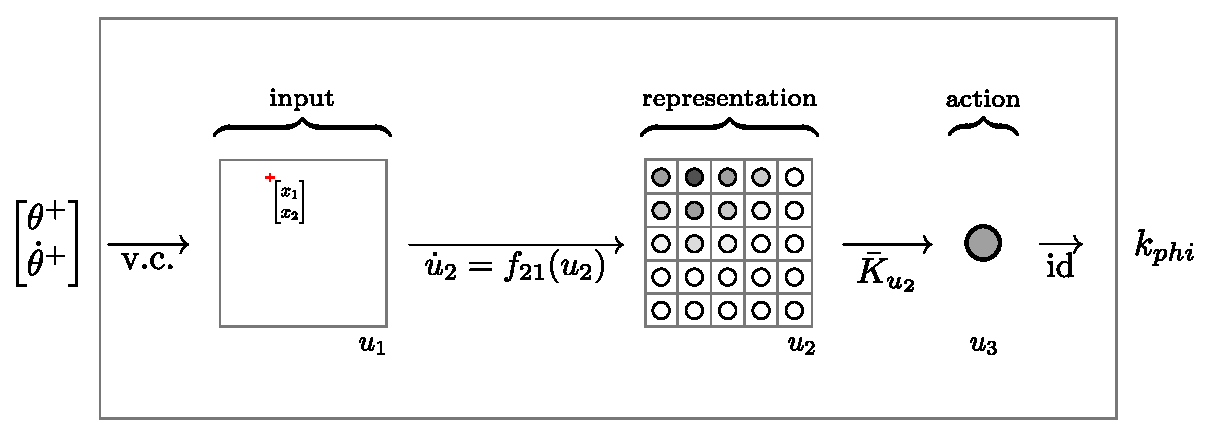
\includegraphics[scale=0.55]{controller_arch_chp3}
  \caption{Neural field controller architecture for Chapter 3.}
  \label{fig:chp3-cont-arch}
\end{figure}

The layers, depicted in figure \ref{fig:chp3-cont-arch} are further
described below:

\paragraph{Input Layer}
This layer is used as a spacial representation of a function of the
inputs, without a dynamic behavior (it does not add state-variables to
the bundled system-controller differential equation). The values
stored in this layer act only as a buffer to feed the inputs to the
representation layer, and correspond in each iteration to a mapping of
the system state-variables. It should be noted that this layer is not
governed by a differential equation and therefore does not follow
Amari's definition of a neural field.

While the mapping function can be general, here it will be
simplified. As a result, the input layer is a direct, vector-coded,
representation of the relevant state of the controlled system after
heel-strike. More specifically, for the input layer population
($i=1$):

\begin{subequations}
  \begin{align}
    u_1(x,t) &= f_I(x,v_n^+) \\
    f_1(x,v_n^+) &=
    \begin{cases}
      \text{const.} & \text{if v.c\,}(v_n^+) = x. \\
      0 & \text{otherwise.}
    \end{cases} \\
    x &= \big[\begin{smallmatrix} x_1 \\ x_2 \end{smallmatrix}
    \big] \in [0,1] \times [0,1] \\
    v_n^+ &= \big[\begin{smallmatrix}
      \theta_n^+ \\
      \dot{\theta_n}^+ \end{smallmatrix} \big] \in [0,0.4] \times
    [-0.4,0]
  \end{align}
  \label{eq:chp3-input}
\end{subequations}

Note that the activation potential of the input layer $u_1(x,t)$ is a
function of the reduced system state-vector $v_n^+$ for the $n$-th
heel-strike (the last occurred at time $t$), and is constant up to the
next heel-strike.

\paragraph{Representation Layer}
The neural population in this layer behaves according to a
differential equation where the input if functions of the activation
potential of the input layer. Therefore, the population in this layer
resembles the definition given by Amari for neural fields
\cite{Amari77Dynamics}, but with an specific structure for the
interconnection between input layer and representation layer
populations, and also, a minor role of recurrence.

The differential equation for the potential at position $x \in
\Omega_2=[0,1] \times [0,1]$ in the representation layer ($i=2$)
population is:

\begin{subequations}
  \begin{align}
    \tau_2\dot{u}_2(x,t) &= -u_2(x,t) + \int_{x' \in
      \Omega_2}{w_{2,2}\left( s_{2,2}(x,x') \right)
      \psi \left(u_2(x',t) \right) dx'} + f_{2,1}(x,t) \\
    f_{2,1}(x,t)&=\int_{x' \in \Omega_1}{w_{2,1}\left(s_{2,1}(x,x')
      \right) \psi \left(u_1(x',t) \right) dx'}
  \end{align}
  \label{eq:chp3-representation}
\end{subequations}

Where as in previous chapters $\tau_i$ is a time constant for the
population $i$, $u_i$ is the activation potential of elements in the
population, $w_{j,i}$ is the connection kernel for connections from
population $i$ towards population $j$, which is a function of
$s_{j,i}$, the distance between two positions (on the same population
$j$, or in different populations $i$ and $j$), $Omega_i$ is the set of
positions $x$ in the layer $i$, and $\psi$ is the activation function
(here a Heaviside function).

The connection kernel $w_{j,i}$ could take any form, but the form of a
Mexican-hat function will be used.

\paragraph{Action Layer}
Similarly as it was done between the input layer, the action layer is
non-differential in nature (so it also does not add state variables to
the bundled system-controller differential equation). Also, it
contains only one node, and its activation corresponds to the
controller output, $k_{\phi}$, the proportional controller constant
defined in section \ref{sec:chp3-simplest}. The mapping between the
representation layer and the action layer ($i=3$) is evaluated using a
weighting matrix, calculated as:

\begin{equation}
  u_3(t) = \frac{\sum_{x'}W_{3,2}(x')u_2(x',t)}{\sum_{x'}u_2(x',t)}
  \label{eq:chp3-action}
\end{equation}

Where $W_{3,2}(x')$ is the estimated control action if the current
state where located in the cell with center at position $x'$. The
actual values for $W_{3,2}$ are assigned to the resulting
$M(\theta_0,\dot{\theta}_0)$ of the search performed in section
\ref{sec:chp3-searching}, which was then assigned directly to
$k_{\phi}$.

\subsection{Insights on the Controller Behavior}

The actual controller that is presented in this chapter may be
understood as a biologically implementation of a Sliding-mode
controller, and works (in general terms) selecting a control policy
for each step, using as
input the Poincar� section \( v_n^+=\big[\begin{smallmatrix}\theta_n^+ \\
  \dot{\theta_n^+} \end{smallmatrix} \big]\). The mapping
$k_{\phi}=M([\theta_n^+ \dot{\theta_n^+}]^T$ is embedded in the
structure of the neural field. The control policy provided as output
by the neural field is the parameter $k_{\phi}$, used as constant for
the locally linear critically-damped PD controller. An interpretation
of the neural field controller structure is detailed next.

The input layer has a two-dimensional (non-dynamic) neural population,
with one dimension for $\theta_n^+$ and another for
$\dot{\theta_n^+}$, the elements in the Poincar� section $v_n^+$ (just
after heel-strike), but rescaled to be in the set $[0,1] \times
[0,1]$. For these populations, the function $f$ in the equation
$u_1(x,t)=f(v_n^+)$ (shown in the previous subsection) performs a
vector coding, i.e. an specific value of the input variable $v_n^+$
causes an activation $u_1(x)$ with amplitude 1 at some position $x$,
and an activation of 0 at any other position. For implementation
purposes, note that this value does not need discretization, as the
input layer is not explicitly modeled, given that it does not add
state variables to the bundled system-controller differential
equation.

The representation layer also a neural population, where the position
$x$ resides in the same two-dimensional space of the input layer
population. An activation of an element of the input layer population
(e.g the one corresponding to $v_n^+$) causes an activation bump that
reaches its maximum at some position in the representation layer, and
decreases as the nodes are farther away. This configuration gives the
representation population an structure that resembles the Poincar�
section space. The implementation has 17x17 elements, an equal number
than that of the mapping found in the section
\ref{sec:chp3-searching}, but it should be noted that the actual
points are different, given that in the position grid of the
representation and input layers each node is located at the center of
each cell, but in the section \ref{sec:chp3-searching} were located at
the cell boundaries.

The output layer has also one population, actually with only one
element, which activation provides the output value $k_{\phi}$. Each
element in the representation layer population contributes with a
value given by the product of its activation potential and the optimal
$k_{\phi}$ value for that position in the approximated Poincar�
section in the representation layer. The total output is calculated as
the average of $W_{3,2}(x')$ wighted by the activation of the
representation layer $u_2(x')$. If $W_{3,2}(x')$ is an approximation
to the optimal control action for state $x'$, and the fraction
$u_2(x',t)/\sum_{x'}u_2(x',t)$ is an approximation to the probability
of being in the state $x'$ at the current time $t$, then this average
provides an approximated expected value for the optimal control action
\(\text{E}_{u_2}\{k_{\phi}\}\).

\section{Results and Discussion}
\label{sec:chp3-results}
The experimental results are shown in the following figures. For
comparison purposes, the State-feedback (SF) control strategy proposed
by Wisse et al. is implemented, and compared to the Optimized
Sliding-mode (OSM) controller developed using search on section
\ref{sec:chp3-searching}, and to the Sliding-mode(-like) Neural Field
(SMNF) controller proposed in the previous section. The experiment
shown is run for $t=[0, 100]$ with the initial configuration \(v_n=
\big[ \begin{smallmatrix} 0.02 \\ -0.39 \end{smallmatrix} \big]\),
which is near the most unstable point in the region studied.

While the SF controller keeps constant the $k_{\phi}=100$ value in
order to attain stability, both the OSM and SMNF controller proposed
recalculate the $k_{\phi}$ (at least) on each step using the current
Poincar� section and the embedded mapping $k_{\phi}=M(v_n^+)$,
directly for the OSM, and indirectly for the SMNF.

The output values of the OSM take the form of a Sliding-mode
controller in the following sense:
\begin{itemize}
\item A subset of Poincar� section at heel-strike defines the section
  of state-space where the system ``slides'' along.
\item At each heel-strike the parameter $k_{\phi}$ is re-evaluated,
  effectively changing the structure of the controller in a
  discontinuous fashion.
\item The matrix of control values $M(v_n^+)$ is built so that the
  system always stays in the subset of the Poincar� section, and
  furthermore, approaches the sliding surface in finite time.
\item Once reaches the sliding surface (fixed point in the Poincar�
  section), the system stays there.
\end{itemize}

On the other hand, the output function of the SMNF uses a weighted
average (analogous to a centroid policy). It interpolates between the
values on the 17x17 mapping grid, but also has a dynamic estimation of
the system state, implemented in the representation layer. The
dynamics of the representation layer could cause the loss of
stability, as it may lag or otherwise underestimate the required
$k_{\phi}$. Nonetheless, as is shown in the figures in this section,
the SMNF (with the kernel function parameters used) approaches quite
closely the behavior in the long term of the OSM controller, but with
a soft and continuous change in the control parameter $k_{\phi}$.

Figure \ref{fig:chp3-activation-movie} shows a sequence of captures,
at increasingly longer intervals, of the activation potential of the
representation layer neural field population. In it can be observed
that the dynamics over the neural field converge as the system
approaches the attractor in the Poincar� section.

\begin{figure}[hp]
  \centering \subfloat[$t=0$ (s)]
  {\includegraphics[width=0.33\textwidth]{cph3-SMNF-activation-t00}}
  \subfloat[$t=1$ (s)]
  {\includegraphics[width=0.33\textwidth]{cph3-SMNF-activation-t1}}
  \subfloat[$t=2$ (s)]
  {\includegraphics[width=0.33\textwidth]{cph3-SMNF-activation-t2}} \\
  \subfloat[$t=5$ (s)]
  {\includegraphics[width=0.33\textwidth]{cph3-SMNF-activation-t5}}
  \subfloat[$t=10$ (s)]
  {\includegraphics[width=0.33\textwidth]{cph3-SMNF-activation-t10}}
  \subfloat[$t=15$ (s)]
  {\includegraphics[width=0.33\textwidth]{cph3-SMNF-activation-t15}} \\
  \subfloat[$t=20$ (s)]
  {\includegraphics[width=0.33\textwidth]{cph3-SMNF-activation-t20}}
  \subfloat[$t=50$ (s)]
  {\includegraphics[width=0.33\textwidth]{cph3-SMNF-activation-t50}}
  \subfloat[$t=100$ (s)]
  {\includegraphics[width=0.33\textwidth]{cph3-SMNF-activation-t100}}
  \caption{Activation potentials for the representation layer
    vs. time, for $t \in {0,1,2,5,10,15,20,50,100}$ (s), for the SMNF
    controller. Centroid marked with a black asterisk (*).}
  \label{fig:chp3-activation-movie}
\end{figure}

\begin{figure}[p]
  \centering \subfloat[$k_{\phi}$ parameter values for the
  controllers.]
  {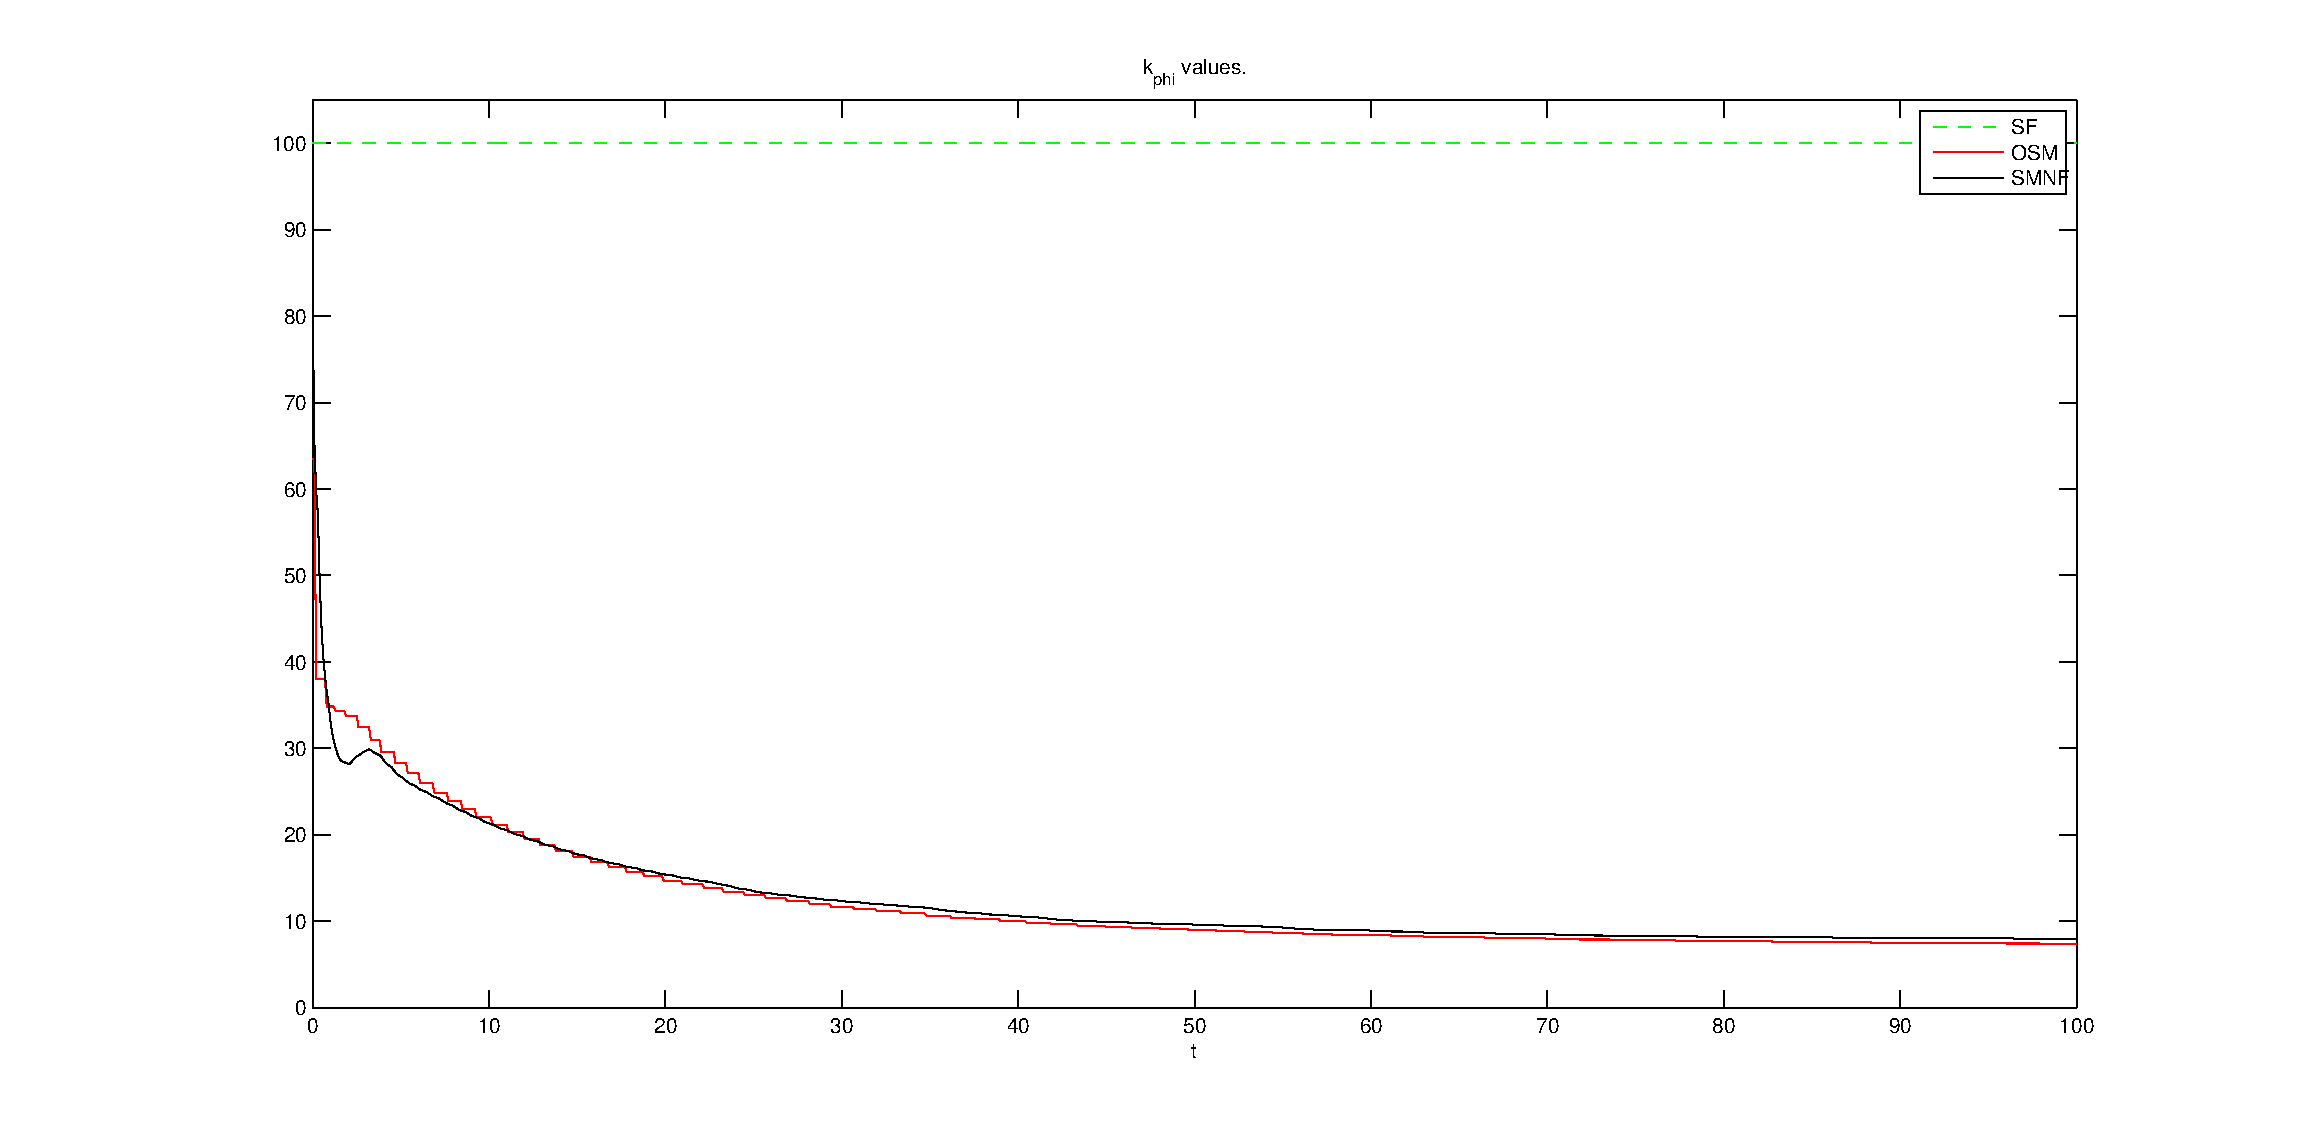
\includegraphics[width=1\textwidth]{chp3-ALL-K-0to100}}  \\
  \subfloat[Integral of squared control action
  ($\int{\tau_{\phi}^2\;dt}$) for the controllers.]
  {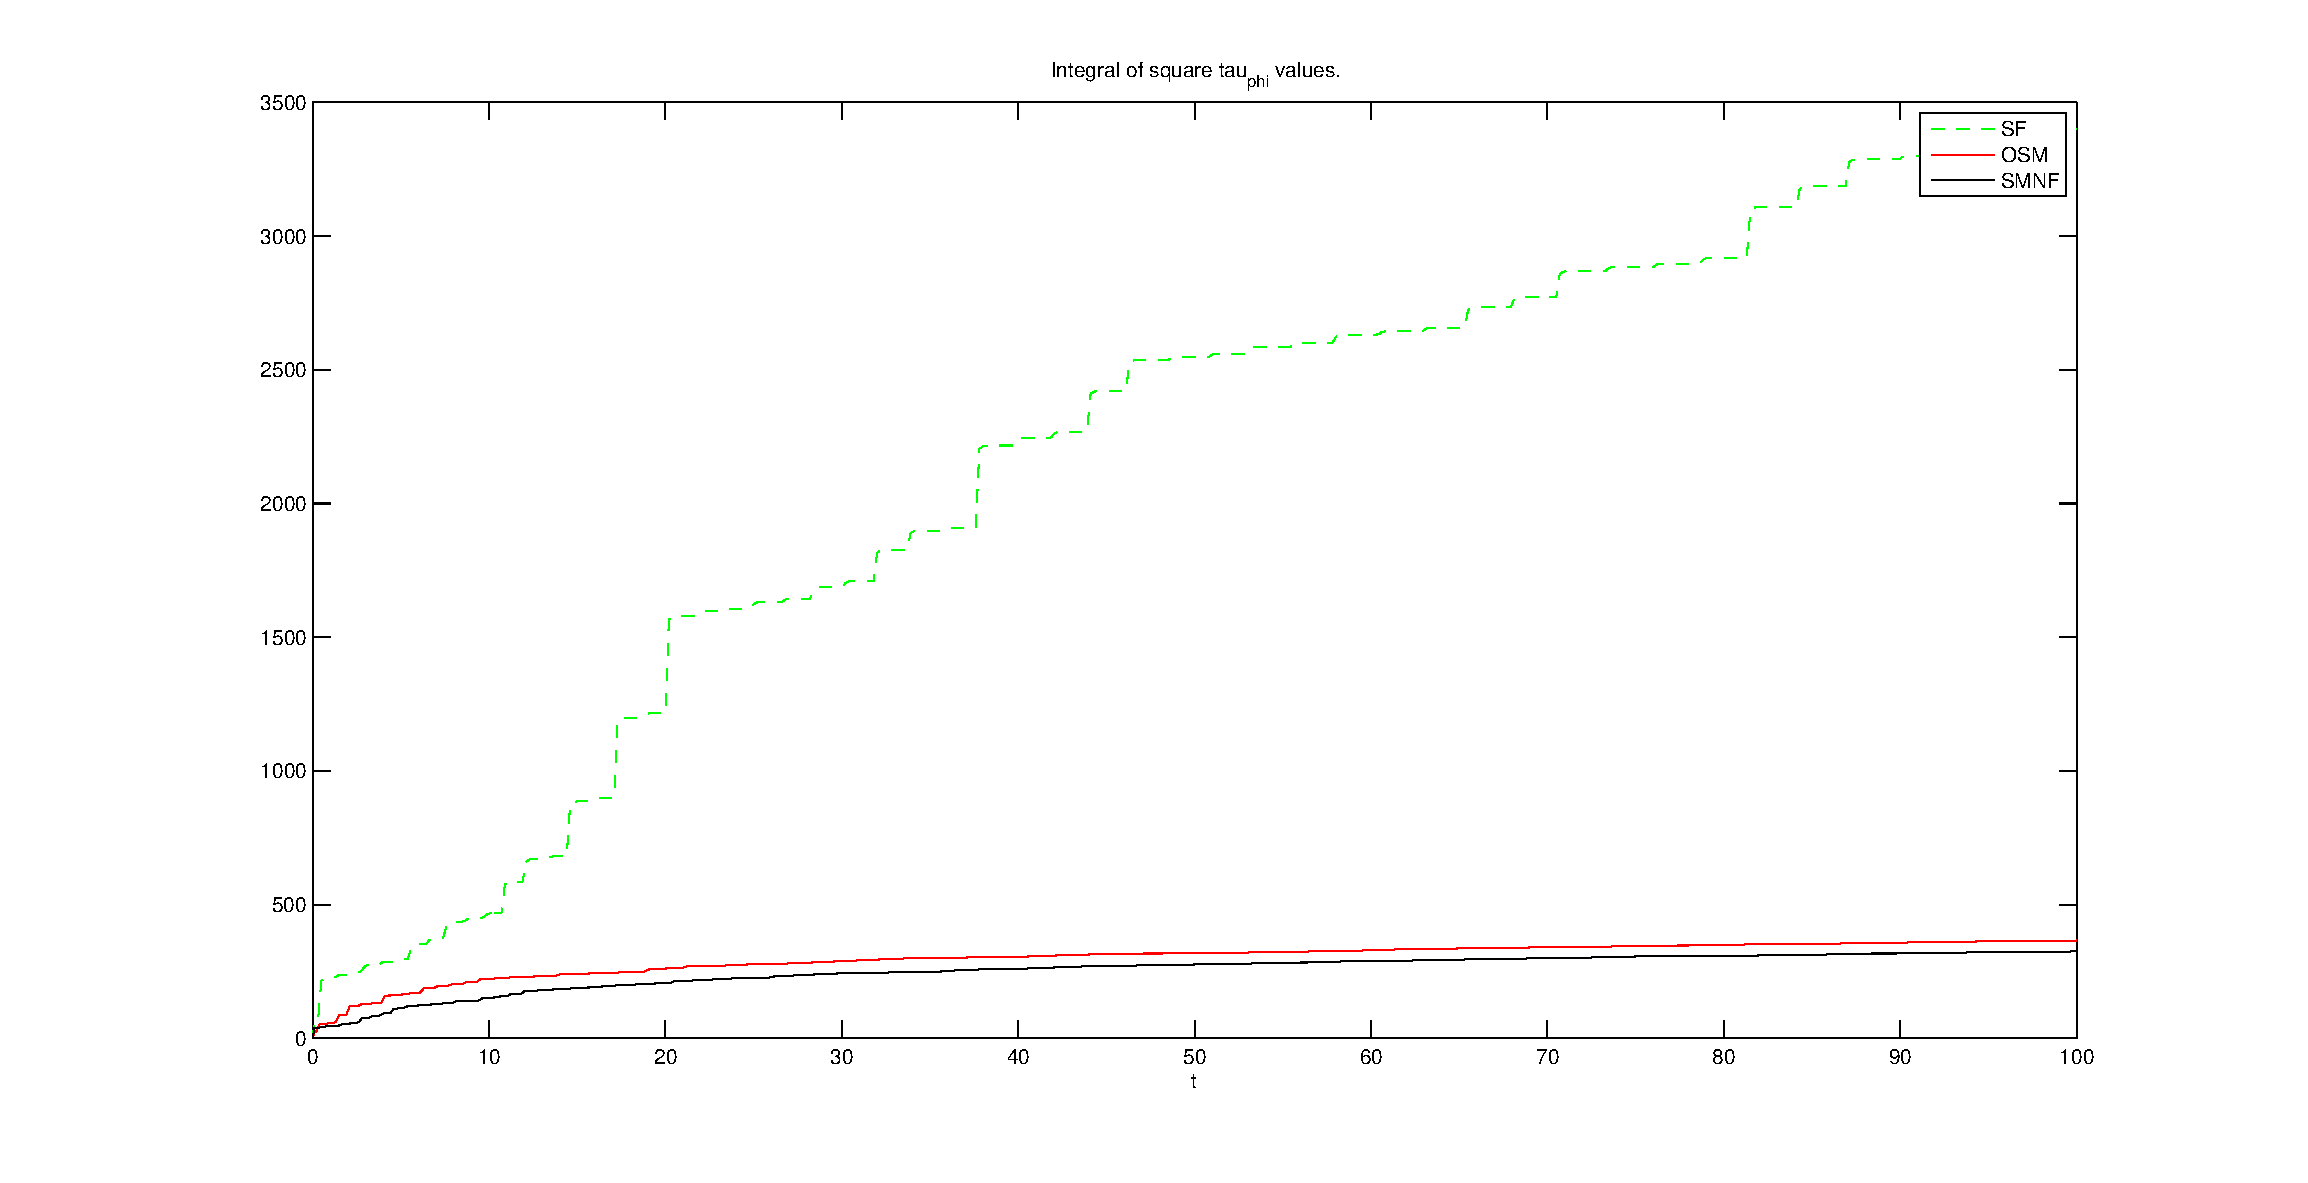
\includegraphics[width=1\textwidth]{chp3-ALL-intTau-0to100}}
  \caption{Controller action vs. time, for $t \in [0,100]$ (s), for
    the three controllers presented in this chapter: Constant
    $k_{\phi}$ for SF controller, step-wise adaptation of $k_{\phi}$
    for OSM controller, and continuous variation of $k_{\phi}$ for
    SMNF controller.}
  \label{fig:chp3-control-action}
\end{figure}

The overall performance of the SMNF controller is better than the SF
in terms of energy consumption and actuator strain, progressively
diminishing its $k_{\phi}$ value and thus the cumulative control
action (see the figure \ref{fig:chp3-control-action} where the
$k_{\phi}$ and $\int{\tau_{\phi}^2\;dt}$ values vs time are
plotted). The SF controller converges faster to its fixed point (as
would be expected for a greater control action), but even in
steady-state the control action stays almost unaltered. On the other
hand, the OSM controller has an slightly higher cumulative control
action than the SMNF controller, but it provides a monotonic decrease
in $k_{\phi}$ across time, behaving more properly as an Sliding-mode
controller.

\begin{figure}[h]
  \centering \subfloat[SF Controller]
  {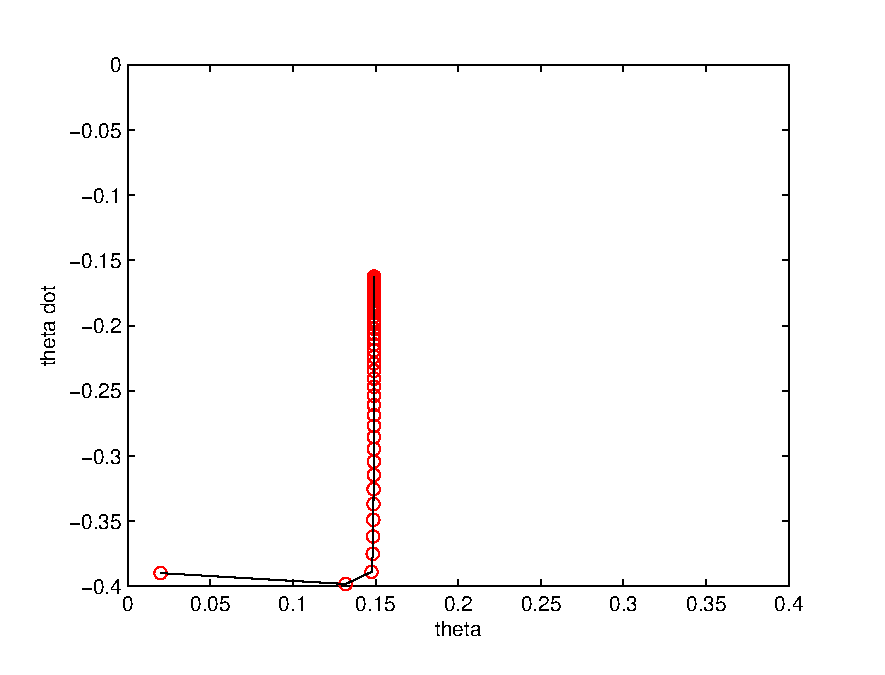
\includegraphics[width=0.6\textwidth]{chp3-SF-PS-0to100}}  \\
  \subfloat[OSM Controller]
  {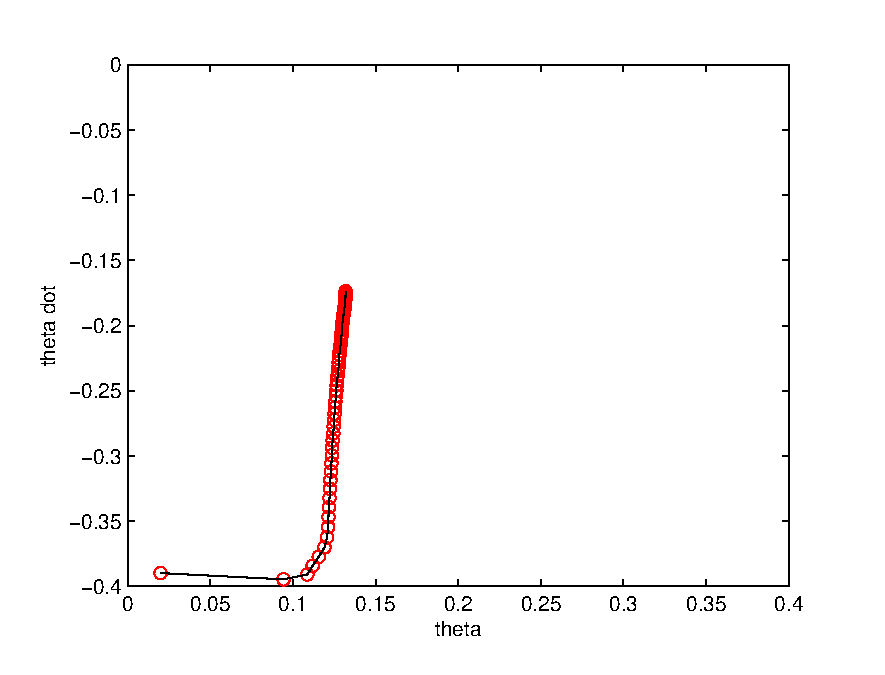
\includegraphics[width=0.6\textwidth]{chp3-OSM-PS-0to100}}\\
  \subfloat[SMNF
  Controller]{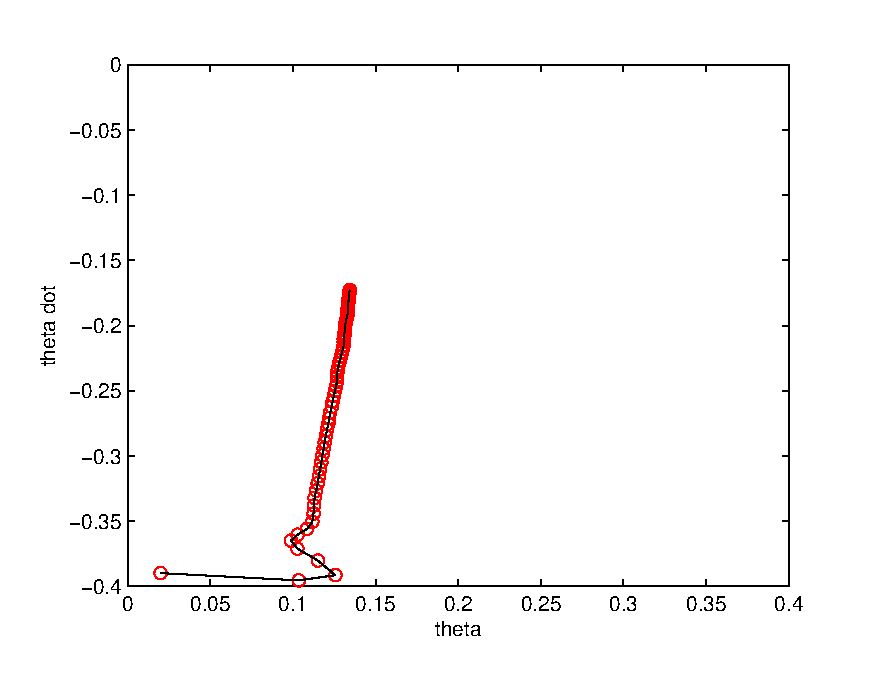
\includegraphics[width=0.6\textwidth]{chp3-SMNF-PS-0to100}}
  \caption{Poincar� Section for the reduced-dimensionality system
    after heel-strike, for $t \in [0,100]$ (s), for each controller
    evaluated.}
  \label{fig:chp3-poincare-section}
\end{figure}

The Poincar� Sections (see figure \ref{fig:chp3-poincare-section}) of
the biped using both the SMNF controller and the OSM controller show
how the system moves from a configuration that requires higher
$k_{\phi}$ values to configurations that require lower ones, and that
fact is exploited by the controllers. The SF controller also moves to
configuration that require lower $k_{\phi}$ values (even closer to the
natural attraction basin of the biped), but that fact remains
unused. This is the main factor of improvement in the controllers
proposed in this chapter compared to the solution of Wisse et al.

\begin{figure}[h]
  \centering \subfloat[SF Controller]
  {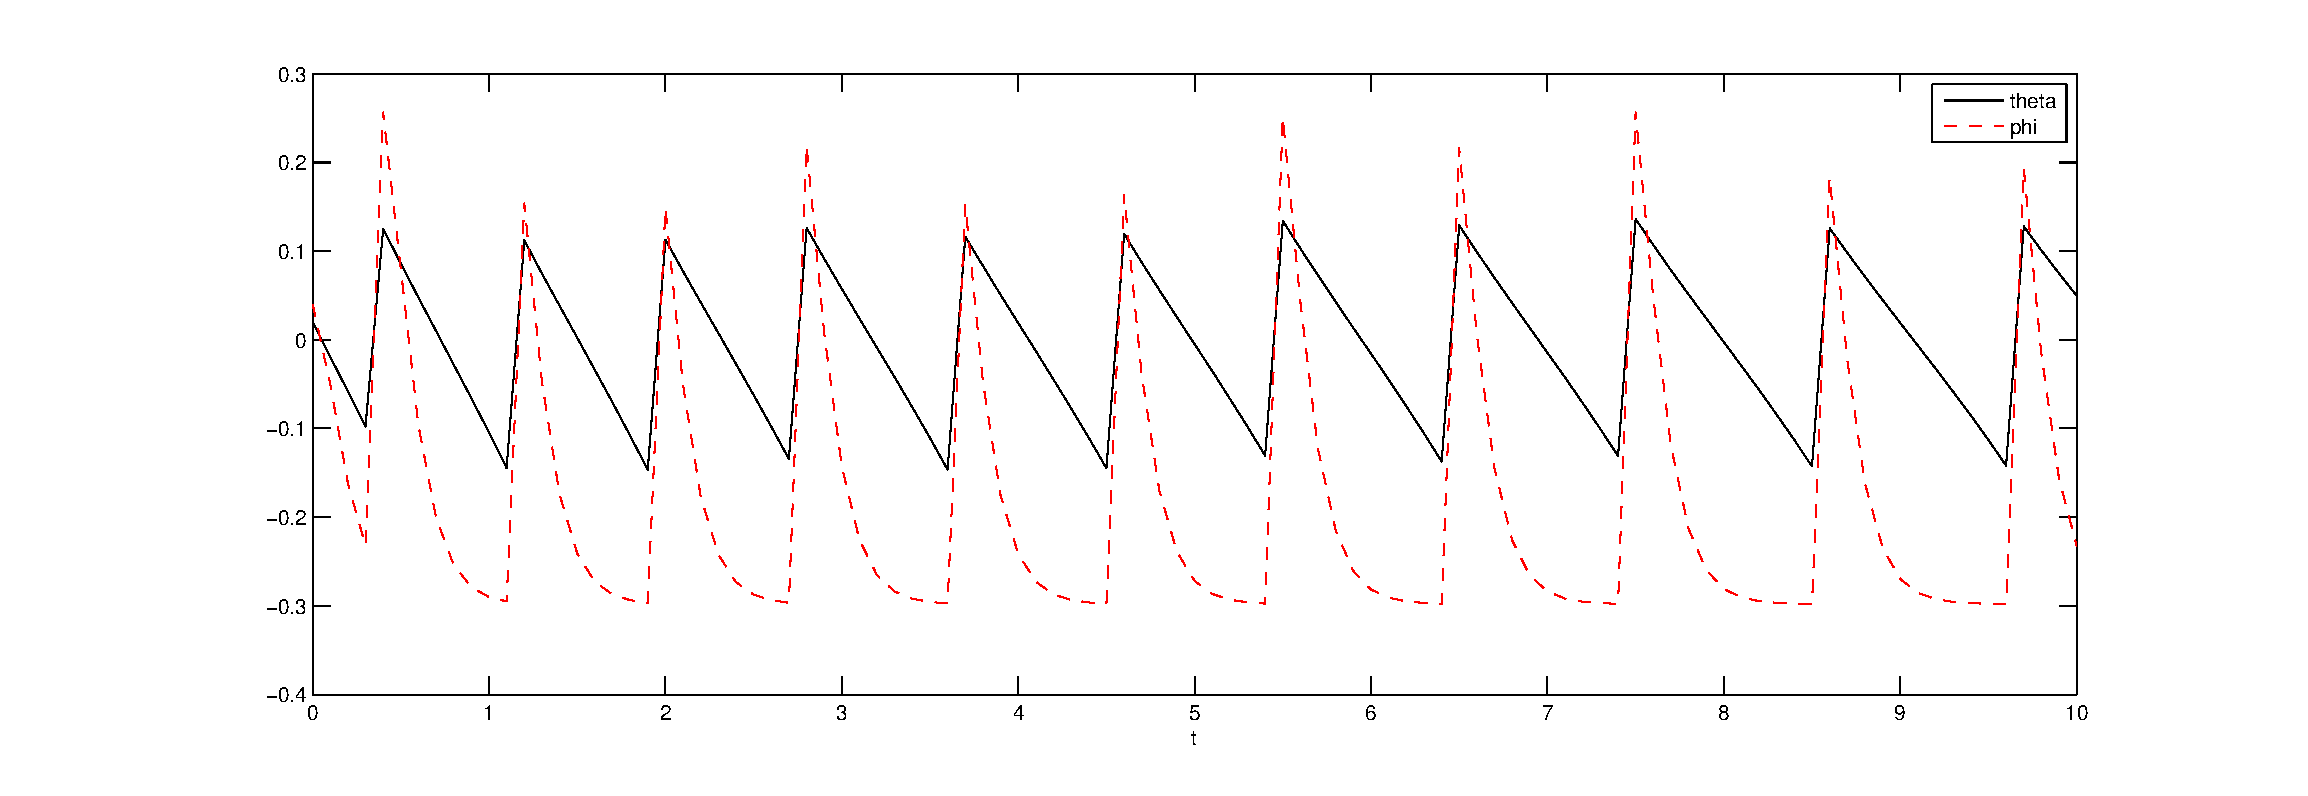
\includegraphics[width=1\textwidth]{chp3-SF-T-0to10}}  \\
  \subfloat[OSM Controller]
  {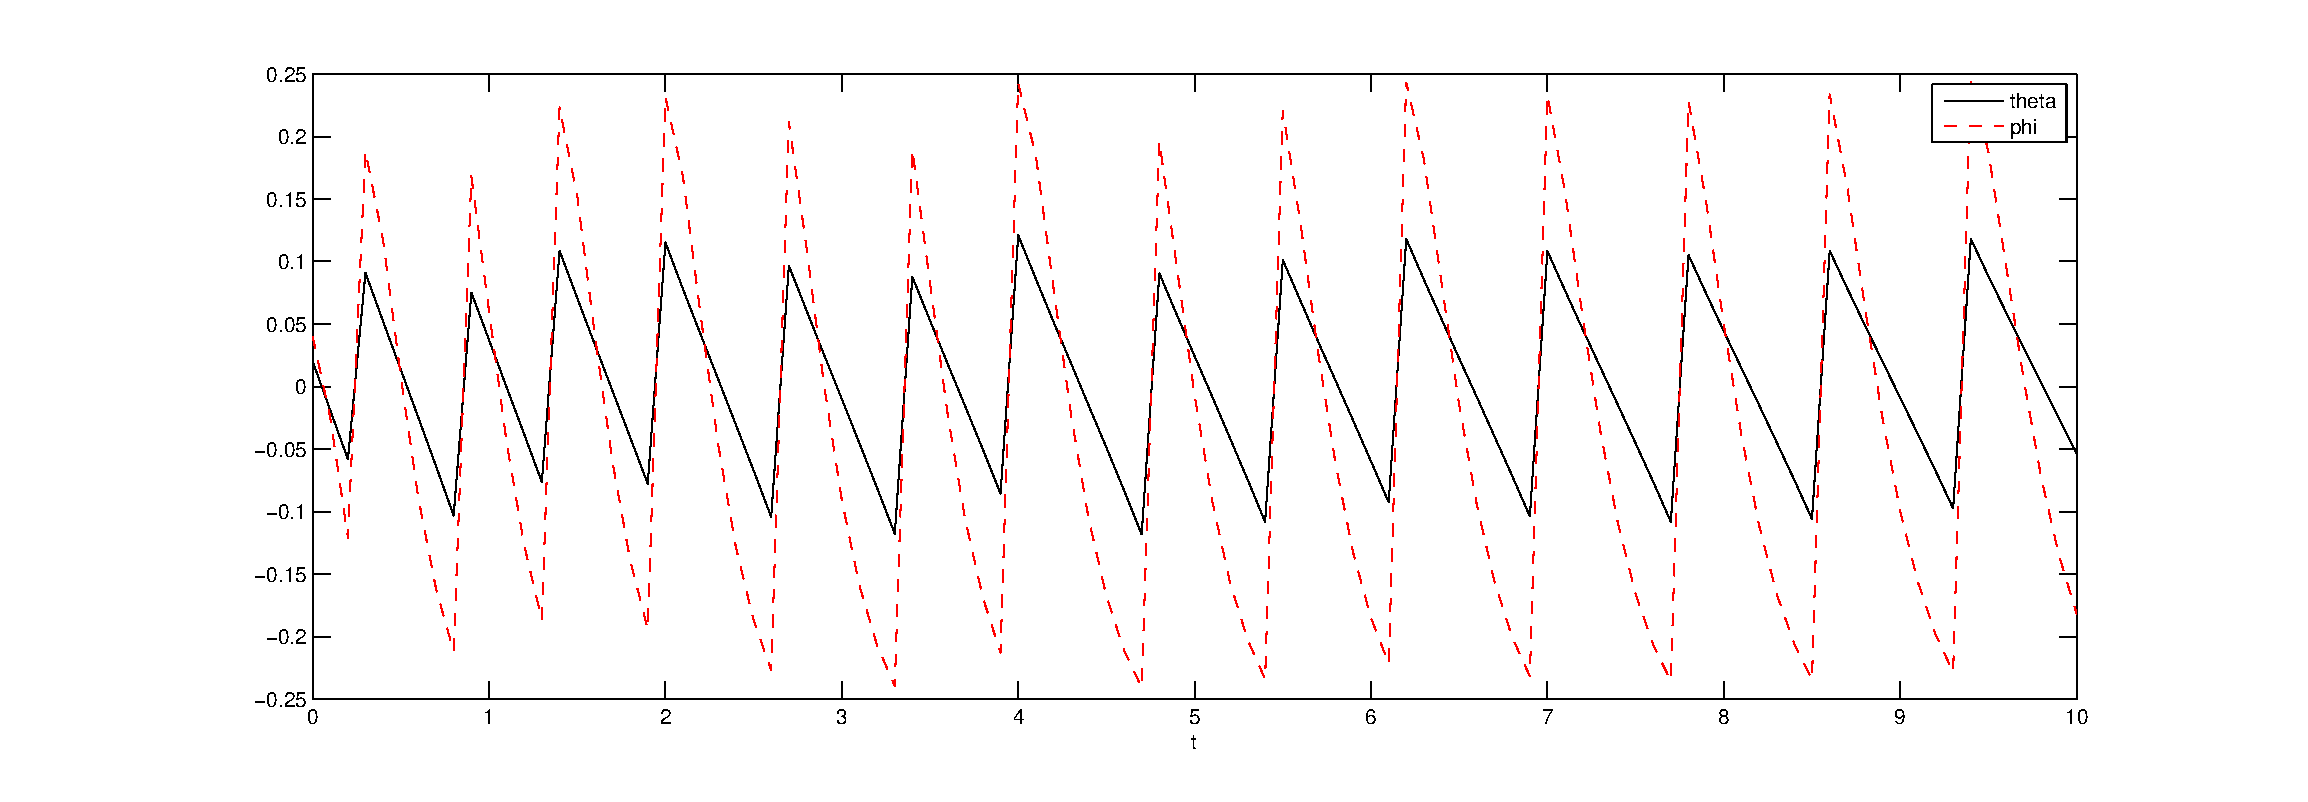
\includegraphics[width=1\textwidth]{chp3-OSM-T-0to10}} \\
  \subfloat[SMNF Controller]
  {\includegraphics[width=1\textwidth]{chp3-SMNF-T-0to10}}
  \caption{System evolution (state variables after heel-strike
    vs. time) for $t \in [0,10]$ (s), for each controller evaluated.}
  \label{fig:chp3-system-evolution}
\end{figure}

The time simulation (see figure \ref{fig:chp3-system-evolution}) shows
how the SMNF changes the control policy (as parametrized by
$k_{\phi}$) softly enough to provide a qualitatively natural gait for
the biped. It should be noted that sudden changes of behavior are
common in Sliding-mode controllers, but that is mitigated in this case
by three facts: 1) The neural field applies an interpolation using the
centroid of activation to calculate the output $k_{\phi}$. 2) The
neural field has natural dynamics qualitatively equal to a low-band
filter. 3) The change in the $k_{\phi}$ occur at a non-linear point in
the biped dynamics that anyway would cause a jump in its state.

In conclusion, in this chapter we presented two controllers which
improve the controller of Wisse et al. over the Simplest Biped Walking
(SBW) model, using a mapping from regions of the Poincar� Section just
after heel-strike \(v_n= \big[ \begin{smallmatrix} \theta_n^+ \\
  \dot{\theta}_n^+ \end{smallmatrix} \big]\) to $k_{\phi}$ values, in
a manner similar to Sliding-mode controllers. Those controllers, while
being active, approach more closely Passive Dynamic Walking (PDW) by
diminishing the cumulative control action. One of the two controllers
proposed is implemented using a control architecture based on neural
fields, which extends and formalizes the structure of the controller
for the inverted pendulum shown in the previous chapter.
%%% Local Variables: 
%%% mode: latex
%%% TeX-master: "thesis"
%%% End: 

